\section{Rootkit Analysis Findings}
\label{rootkit_analysis}
% several rootkits analyzed: module_hide (change module linked list), taskigt (create proc files)
%		still to port: change system call table (difficult in kernel 2.6)
% analyze the changed toplevel symbol names
% analyze all symbol names
For each analyzed rootkit a snapshot has been taken before installation and after and the changed kernel symbols were listed.
We used this information to first of all check if
malicious behaviour of each different type of rootkit is reflected among all the changed symbols.
The following sections present our findings.

\subsection{Rootkit Types}
For a rootkit it is not only important to implement some specific services needed by the attacker, but 
also to make those capabilities accessible. At the same time the malicious module wants to hide itself 
and all its activities from the system administrator. To accomplish this, several hooking mechanisms 
into the kernel have to be established. Among the rootkits, that are public available, there are basically 
three different mechanisms of hooking into the kernel. One is to generate special files in the 
Virtual File System (VFS) like \texttt{proc}, another one is to modify kernel structures directly and 
the third and most commonly used one is to replace specific system calls in the system call table (\texttt{sys\_call\_table}).	

\subsubsection{System Call Replacement}
\label{system_call_replacement}
When using an operating system, 
the user must be able to perform system calls in order to invoke special kernel functionalities (for example listing 
and opening files). For this purpose the linux kernel manages a big array with function pointers to the system call 
functions implementing each functionality. 

If a programm invokes a system call (interrupt \texttt{0x80} on x86 architectures), the interrupt dispatcher looks up 
the desired function in the \texttt{sys\_call\_table} and calls it. Until kernel version 2.6 the \texttt{sys\_call\_table} 
was among the exported symbols that could be used by loadable kernel modules. Therefore it was easy to replace the 
function address by an address of a function that intercepts the system call to, for example, filter out specific 
files from directory listings in order to hide the rootkit itself. 

Since Kernel 2.6 the syscall table symbol was no longer exported and the rootkit authors had to invent new ways 
of finding the table location:

\begin{enumerate}
	\item {\b Kernel Memory Search}: With this method the memory area between \texttt{init\_mm.end\_code} and 
		\texttt{init\_mm.end\_data} (which is basically the \texttt{\_text} segment of the kernel image), 
		is searched and the contents are compared to the addresses of known system call functions. 
		Since we know where the specific system call function, we searched for, is located in the system call table, 
		we can calculate the start address.

	\item {\b Interrupt Handler Search}: On the x86 architecture there exists the \texttt{sidt} instruction. 
		This instruction gives us the address of the interrupt vector table. We know that for calling a system call 
		the \texttt{0x80} interrupt is raised and the appropriate interrupt handler calls the right system call 
		function for us. Since the handler has to know there the table with all the system calls is located, 
		we can search in the memory section, where the handler resides for the actual function call and extract 
		the start address of the \texttt{sys\_call\_table} from there.

	\item {\b Compile Time}: A third technique is to use the address known from \texttt{System.map} at compile time. 
		In this case we have to be able to compile our rootkit on the machine where we want it later to be run. 
		We also have to have access to the \texttt{System.map} to lookup addresses. Eventually a module
		could also find out the syscall table address at load by looking it up in \texttt{/proc/kallsyms}.
		In our tests this is the method we used.
\end{enumerate}

On newer 2.6 kernels it is not sufficient to find the system call table. Several protection mechanisms have been employed: 
The pages where the table resides is flagged as read only. 
Trying to change that with the \texttt{set\_memory\_rw} function will fail since this function also has some 
protection built in. But a kernel hacker is still able to modify this part 
of memory: Since we cannot use the kernel functionality to change access rights of memory sections, we have to implement 
them ourselves. Walking the page tables and changing flags could be implemented in the loadable kernel module itself.

Detection of such modifications are possible with our tool. It detects all changed function addresses in the table. 
One rootkit we inspected did even go further than just replacing function pointers: It did not replace the system call 
table itself, but it first copied it and modified the copy. Then the interrupt handler for system calls was modified 
to use the new system call table. Such a modification is not yet detected by our tool, since we do not yet take
registers into account as global symbols. Thus the tool still uses the address 
of the old table, which stays unmodified. If we are inspecting a virtual machine the machine registers have to be
considered as well.

\subsubsection{VFS Manipulation}
The virtual file system is an additional layer on top of all the file systems implemented in Linux. 
It enables the user to uniformly access his files independently of the underlying file system. One special 
file system present in Linux, is the \texttt{proc} filesystem. It was implemented to give access to 
kernel and loadable module parameter configuration or to access debug information present in the kernel. 

The file entries in the proc file system are different from ordinary files. On access of such an entry, 
there is no read from a block device. Instead a function call to a specific function associated with that 
file node is called. Within this function the neccessary data can be generated and copied back to the user. 
Analog happens upon write access to the file. The data written by the user can be parsed and configuration 
parameters can be set accordingly.

One rootkit we analyzed used VFS manipulation to give root privileges to certain processes. To accomplish 
that a new file is created in the \texttt{/proc} directory. If a process accesses this file, the kernel function 
handling the read or write operation has access to a \texttt{task\_struct} structure of exactly that process. 
Therefore it is easy to modifiy the \texttt{uid, gid,...} members of that structure, which control the privileges.

Detection of such a modification can be done using our toolkit. The difficulty in this case lies in the 
classification of the changes. In our experiments we observed numerous proc filesystem modification during normal 
operation of the running machine. Just creating an entry in /proc is not neccessarily malicious. Changing the 
UID of a process can be, but can also happen during normal runtime (take \texttt{sudo} for example). 
Therefore unauthorised modification is very difficult to spot. One can try 
to match malicious behaviour by inspecting the filenames of the newly created files, but this name can easily 
be changed to something unsuspicious by the attacker.

\subsubsection{Direct Kernel Object Modification}
Most of the rootkits did hide themselves by system call interception 
and filtering of the results as described in section \ref{system_call_replacement}. 
Another technique is to modifiy the kernel structures directly. Of course malicious 
attacks other than just hiding can be achieved with direct kernel object modification.

\begin{figure}[htb]
	\begin{center}
	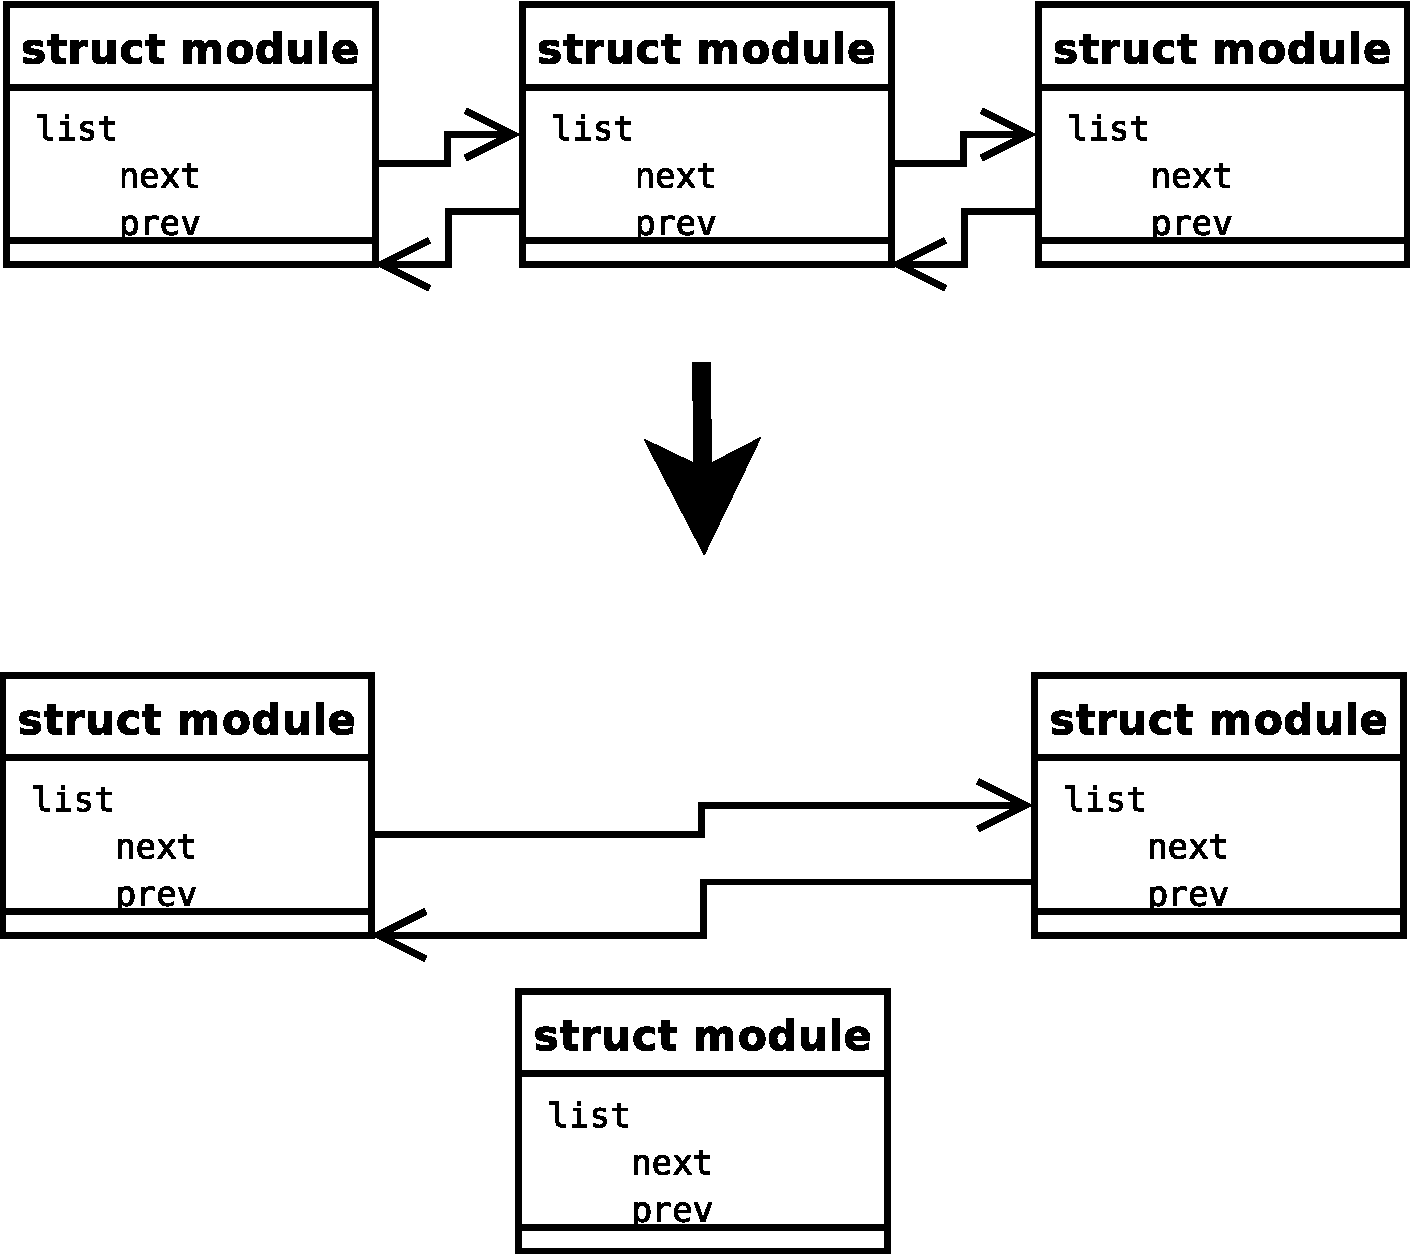
\includegraphics[width=0.45\textwidth]{imgs/module_list_modification.pdf}
	\caption{Skipping a module in the internal kernel module list.}
	\end{center}
	\label{skip_module}
\end{figure}

For keeping track of all the loaded modules, the kernel manages a double linked list. The kernel system 
calls that deal with modules (e.g. \texttt{insmod}), make use of this list. 
If the user requests to unload a specific module from the kernel, first the module list is searched 
for one with the specified name, then this reference is taken, unloaded and removed from the list.

If the attacker now removes a specific module (see figure \ref{skip_module}) from the internal list, by just 
updating the pointers (see figure \ref{skip_module}) and thereby skipping one entry in the double linked list, 
the kernel itself has no more access to this. Removing and other access to this module is no longer possible. 
Also the module does not show up on \texttt{lsmod}, which was the intention of the modification. 
Another fact is that all the hooks and callbacks, the malicious module may have placed into the kernel, still exist 
and the module itself still resides in memory. Therefore the normal operation of the rootkit is available, while 
unloading and listing is not possible.

Detecting such modifications is possible with our toolkit. We are able to monitor all changes of kernel structures. 
For double linked lists, the list has to be traversed and all the entries analyzed (though the current version 
still has some problems fully dealing with linked lists). To be able to successfully detect an attack on kernel 
structures, we have to further analyze the changes. It could be possible that the module list has changed, 
because we loaded a kernel module by hand. These kind of changes have to be filtered out. 

Another difficulty in detecting such modifications are big timesteps between two analysis. If we take one 
snapshot before the malicious rootkit is loaded and one far after the module is completely loaded and 
already hidden, then we will see no changes in the module list. The module already vanished and cleaned 
itself up, leaving no direct traces for us to analyze. We still can search the memory for placed hooks 
into the kernel, which have to be there in order for the rootkit to function correctly.

\subsection{Analysis Conclusions}
Most of the modifications done by the studied rootkits can be identified with our method. 
The big challenge is to distinguish between malicious and normal changes of kernel structures. 
In the case of proc file system modifications we could find 
more modifications by just running a xterminal with some commands then by inserting the tested rootkit.

When supervising a virtual machine, it is also neccessary not only to monitor the memory, but also the special registers 
of the virtual cpu. Then even modifications of the interrupt handlers and with that copies of the system call table can 
be detected.
